
\chapter{First Experiment}

\todo[inline]{Todo capítulo deve ter uma introdução explanatória. "This chapter describes"}

\todo[inline]{Acho que pode até ser Primeiro Ciclo, ou pode ter um nome como ``Efetividada das LLMs na Solução..''  vai ter que quebrar esse capítulo, que tem muita informação nos conceitos da DSR: no mínimo nos quatro principais: Contexto, Problema, Artefato, Avaliação. Grande parte do contexto e problema já devem ser descritos no capitulo que eu pedi para criar e aqui só faz referência.}


\todo[inline]{Ok, você foi direto para o experimento mas não disse o que ia fazer. Aqui exatamente cabe o quadro da DSR que eu te mandei: qual o contexto, qual o problema, qual a suposição (de utilidade ou de mundança de contexto), qual os quadro teóricos, qual o(s) artefato(s) proposto(s) e como serão avaliados, vai fechar muito bem.}
    

    \section{Methodology}

            This section describes the approach and tools employed to investigate the effectiveness of a language model-based agent in responding to specific queries within the domain of well construction and maintenance\xexeo{isso aqui é a validação, mas qual é o problema, qual a proposta, são essas informações que faltam para ficar bem organizado}. 
            Firstly, the preparation, selection, and utilization of the data sources are described, explaining how each contributes to the knowledge base from which the agent derives its responses. 
\todo{inline}{Aqui seria bom fazer um BPMN do passo a passo do seu experimento, veja a figura 4.1 de\url{https://www.cos.ufrj.br/uploadfile/publicacao/3172.pdf}}

        \vspace{5mm}
        \subsection{Data Preparation.} 

            This experiment was carried out in the well construction department of a major oil company\xexeo{Olha o contexto aqui}.
            The choice of tasks focused on technical knowledge management and data analysis\xexeo{Contexto e problema?}. 
            Examples\xexeo{Exemplos? Não são todas? Quantas foram? Por que foram escolhidas? Tem que explicar como foram criadas essas queries, do jeito mais honesto possível, mesmo que seja pela experiência do autor, por pergunta a colega ou consulta uma coleção de documentos com perguntas e respostas. Tem que listar todas. Se foram MUITAS mesmo, coloca em apêndice.} of queries used in the experiment are listed in Table~\ref{table:question_examples}\xexeo{Isso aqui é a exemplificação do problema, aliás, dava até para falar um pouco da criação de datasets de teste lá na revisão da literatura}.        


            
            The data sources for executing such tasks were chosen to cover a range of operational scenarios in the activity of well construction and maintenance: Operational Knowledge Items, Operational NPTs (Non-Productive Time), and a Collaborator Finder. 

\xexeo{para claridade, eu  separei as linhas da tabela 3.1 com linhas físicas, mas mudei a forma que você estava formatando.}

            % [TENTAR INCLUIR EXEMPLOS DE PERGUNTAS]
            \begin{table}[h]
                \centering
                \sloppy
                \begin{tabular}{|p{.2\linewidth}|p{.8\linewidth}|}
                    \hline
                    \textbf{Task category} & \textbf{Query example} \\   \hline
                    \multirow{9}{*}{Q\&A} & How does the presence of silica in the composition of cement 
                    paste affect its thermal stability at high temperatures? \\ \cline{2-2}
                    & What are the main challenges and risks associated with through tubing plug and abandonment in highly deviated wells? \\ \cline{2-2}
                    & What can cause hydrate formation in the Tree Running Tool  connector during the HCR (High Collapse Resistance) hose flush  before connecting to the Wet Christmas Tree? \\ \cline{2-2}
                    & What can cause the Down Hole Safety Valve to remain open  due to hydrate formation in the control lines? \\ \cline{2-2}
                    & What can cause damage to thread protectors and sealing  areas of pin ends of pipes stored at the coating yard? \\ \cline{2-2}
                    & What can cause high drag and torque off-bottom during  the drilling of a well with high deviation? \\ \cline{2-2}
                    & What precautions should be taken when performing a top check  of the abandonment plug in wells with higher inclination? \\ \cline{2-2}
                    & What are the critical factors to consider when choosing a base  fluid for manufacturing a viscous support plug? \\ \cline{2-2}
                    & What are the best practices for managing drilling parameters  during cement cutting to avoid premature bit wear? \\ 
                    \hline                
                    \multirow{2}{*}{Text-to-SQL} & What was the longest-lasting NPT on rig number 05? \\ \cline{2-2}
                    & How many NPTs occurred on rig number 06 during August 2023? \\ 
                    \hline
                \end{tabular}
                \fussy
                \caption[Query examples used in first cycle.]{Query examples used in first cycle. }
                \label{table:question_examples}
            \end{table}




            \emph{Operational Knowledge Items}: during drilling, completion, and workover interventions, documents called Knowledge Items are written by specialists, as depicted in Fig~\ref{fig:report_example}, which can be of 4 types: Technical Alert, Learned Lesson, Good Practice, and Well Observation. 
            This is a tool for knowledge management, considering the large number and variety of specialists involved and well operations performed.\xexeo{\textbf{Essas explicações sobre o que são os documentos podem vir no capítulo que explica a área e configurar o contexto do DSR}}
            
            \emph{Operational NPTs (Non-Productive Time)}: the second data source refers to data on anomalies that occurred during well interventions, containing information such as the title, description of the event, the well where it occurred, type of operation, responsible sector, involved rig, lost time in hours, and start and end dates of the event. 
            These data are critical for the industry, as NPTs represent periods when the operation of drilling, completion or maintenance is interrupted due to some technical or logistical problem. The identification and analysis of these events are essential for continuous process improvement, cost reduction, and increased operational efficiency. By understanding the causes and circumstances of these incidents, organizations can develop strategies to prevent them in the future, optimizing operation time.\xexeo{capitulo da area}
            
            \emph{Collaborator Finder}: the third data source used in the experiment is a collaborator finder, an important tool within an organization for consulting and managing employee data. 
            This system allows for quick search and identification of employees through information such as name, workplace, company, registration, and role. The importance of this tool for the experiment lies in the possibility of cross-referencing employee data with other information sources for a more complete response by the agent.\xexeo{capitulo da area}
            
            Each of these sources provides inputs for the agent to offer a more accurate and updated view of operations and organizational structure.
            A set of documents and records was randomly selected from each database, over which questions were formulated. For each document, up to 3 questions were generated, resulting in a dataset of tasks of the Q\&A and Text-to-SQL types. Some examples are described in Table \ref{table:question_examples}.\xexeo{revisar para fazer sentido as coisas virem de outro capítulo}


        % \vspace{5mm}
        % \textbf{Document Embedding and Semantic Information Retrieval.} 
        %     One data source used by the agent in this experiment is accessed through semantic retrieval.
        %     For this purpose, each document is subjected to an embedding model, text-embedding-ada-002 \citep{OpenAI2023}, which generates a vector with 1536 dimensions that semantically represents the content of the document.
        %     Each document, along with its semantic vector, is saved in a Vector Store database called \citep{Qdrant2024}.
        %     This tool, when presented with a new semantic vector related to the user's query, retrieves the N documents with the highest similarity, i.e., those whose vector is closest to the vector of the content being searched.

        % \subsection{Single-Agent Architecture with Multiple Tools}
        % \vspace{5mm}
        % \textbf{Single-Agent with Multiple Tools.}   
            In this work, a goal-based agent\xexeo{Se certificar que estão descritos na revisão da literatura, caso contrário descrever lá} \citep{Russell2020} was implemented with the goal of accurately responding to various queries. 
            The agent operates within an environment equipped with multiple tools for task-specific operations, as shown in Figure~\ref{fig:agent_environment}, and interfaces with users to receive queries.
            
            \begin{figure}[h]
                \centering
                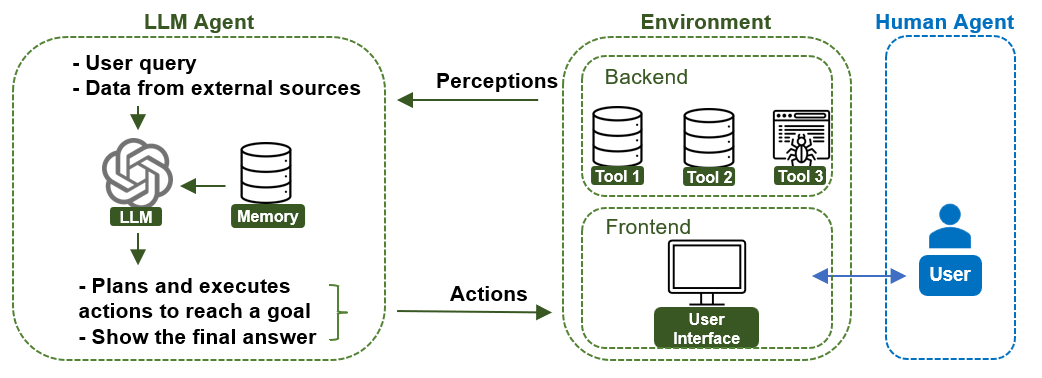
\includegraphics[width=0.75\textwidth]{images/agent_environment_4.png}
                \caption{Schematic of the LLM-based agent interacting with an environment containing tools for task-specific operations, and the Human Agent interface for user interaction and feedback.}
                \label{fig:agent_environment}
            \end{figure}           
            
            Initially, a configuration of agents was implemented as described in Figure~\ref{fig:agent_config_1} using AutoGen Framework \citep{Wu2023} with an architecture that allows information retrieval and user interaction. This system consists of\xexeo{of ... melhor dizer two alguma coisa?}:

            \begin{figure}[h]
                \centering
                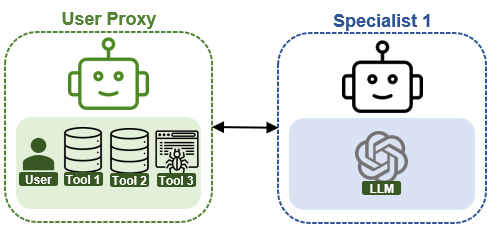
\includegraphics[width=.5\textwidth]{images/agent_config_1.png}
                \caption{Chat setup with one User Proxy \citep{Wu2023} and one Assistant.}
                \label{fig:agent_config_1}
            \end{figure}
            

            \begin{itemize}        
                        
                \item \textbf{User Proxy:} represents the interface with the user and with tools to access external databases. The modular nature of the tools allows the User Proxy to be customized and expanded based on the variety of data sources and the specific requirements of the application domain.

                \item \textbf{Agent:} powered by LLMs such as GPT-4 and GPT-3\xexeo{Aqui tem que dizer que é configurável, só ficou claro para mim mais tarde na leitura}, is the analytical engine of the system. This agent interprets the queries received from the User Proxy and formulates responses.
                                    
            \end{itemize}

            
            For each question in the data set, the agent's decision-making process is executed as described in Figure~\ref{fig:diagrama_agente_1}, initially selecting the appropriate tool to respond to a query and, finally, compiling the retrieved information to provide a final answer.
            
            \begin{figure}[h]
                \centering
                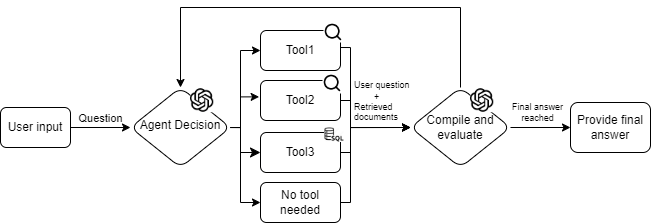
\includegraphics[width=0.75\textwidth]{images/agent_diagram_1.png}
                \caption{Decision process of the agent.}
                \label{fig:diagrama_agente_1}
            \end{figure}                        
                    
            In this experiment, three tools were considered in the decision-making process:

            \begin{itemize}
            
                
                \item \textbf{Tool 1 - Knowledge Items Search:} a tool to search for learned lessons that may be relevant to the query. 
                \label{Tool1}
        
                \item \label{Tool2} \textbf{Tool 2 - Employee Search:} functionality that allows the search for information related to collaborators of an organization.
        
                \item \label{Tool3} \textbf{Tool 3 - NPT SQL Query:} Interface for executing SQL queries on a database of operational NPTs.    
                
            \end{itemize}

            In parallel, there is a pathway that allows the LLM Agent to provide a direct response, without the need to resort to other tools, presumably used when the agent already possesses the necessary information. 
            Finally, the agent presents the final response to the user, which is the product of a language model processing, taking as input the user's query and relevant information retrieved and included in the context of the prompt.

             Table~\ref{tab:tabela_inputs} provides a detailed analysis of the performance and accuracy of different models, specifically GPT-3.5-turbo and GPT-4, when queried about the impact of silica on the thermal stability of cement paste at high temperatures.\xexeo{Por que essa pergunta? Isso é um exemplo? Como o multi agente entrou aqui se ainda não falou de multi agente? Melhor deixar para mais tarde ou mostrar só para single-agent?} 
             The table compares both single-agent and multi-agent setups, evaluating the final outputs based on truthfulness, performance, and specialist comments. 
             For each query, the table highlights the relevance and accuracy of the information provided by the models, including any extraneous or unrelated sections noted by the specialists. 
             This \xexeorem[comprehensive]{OLHA UMA PALAVRA INÚTIL TÍPICA DE LLM} comparison allows for an \xexeorem[in-depth]{Outra} assessment of the models' capabilities in generating accurate and relevant responses to technical questions.

            \begin{landscape}
                \begin{table}[h]
                    \small
                    \centering
                    \caption{Query sample with inputs, outputs, and evaluations.}
                    \label{tab:tabela_inputs}
                    \begin{tabular}{| m{3cm} | m{1.5cm} | m{1.5cm} |>{\scriptsize}m{9cm} | m{1.3cm} | m{1.2cm} |>{\scriptsize}m{4cm} |}                    
                    \toprule
                    % \textbf{Input query} & \textbf{Model} & \textbf{Setup} & \textbf{Final output} & \textbf{Truthfulness} & \textbf{Performance} & \textbf{Specialist \ Comments} \\
                    Input query & Model & Setup & Final output & Truth. \newline fulness & Perfor- \newline mance & Specialist \ Comments \\
                    \midrule
                    How does the presence of silica in the composition of cement paste affect its thermal stability at high temperatures? & GPT-3.5-turbo & Single-Agent & The presence of silica in the composition of cement paste can affect its thermal stability at high temperatures due to some characteristics of silica. Silica is an inorganic material that has a stable crystalline structure at high temperatures. When exposed to high temperatures, the silica present in the cement paste can undergo structural transformations, resulting in changes in the properties of the paste.

                    One of the main changes that can occur is the thermal expansion of the cement paste due to the formation of unstable silica compounds. This thermal expansion can lead to cracks and fissures in the structure, compromising the material's integrity and stability.

                    Moreover, the presence of silica in the composition of cement paste can affect the material's thermal resistance. Silica has low thermal conductivity, which can lead to a reduced ability of the cement to withstand high temperatures. This can result in a decrease in the material's strength and, consequently, a reduction in its thermal stability.

                    In summary, the presence of silica (...) & 4 & 5 & Created a section that is irrelevant to the question: "Moreover, the presence of silica in the composition of cement paste can affect the material's thermal resistance. (...)" \\
                    \cline{3-7}
                    &  & Multi-Agent & The presence of silica in the composition of cement paste has a positive effect on thermal stability at high temperatures. Silica is added to cement to mitigate the retrogression of cement strength when exposed to temperatures above 230°F (110°C). Deep wells or those with a high geothermal gradient may require the use of silica cement to ensure the thermal stability of the paste. The use of silica cement is particularly important in surface casing cementing, where the temperature can exceed the critical limit. \ (...) & 2 & 2 & Retrieved an unrelated Lesson Learned on the subject (about plugs). \\ 
                    \cline{2-7}
                    & GPT-4 & Single-Agent & The presence of silica in the composition of cement paste increases thermal stability, especially at high temperatures. Silica is used to transform the cement into a refractory material, capable of withstanding extreme conditions. 
                    
                    The cement (...).

                    However, (...). & 3 & 4 & Although it is true, the item on the side is not relevant to the question: "However, it is important to note that (...)." \\
                    \cline{3-7}
                    &  & Multi-Agent & Silica is added to cement at a ratio of 35\% by weight of cement to mitigate the retrogression (loss of compressive strength) of the cement in the well when subjected to temperatures above 230ºF (110ºC). \ (...) & 5 & 4 & Cited an unrelated (but true) Lesson Learned about plugs, Lesson Learned LA7005. \\
                    \hline
                    \end{tabular}
                \end{table}
            \end{landscape}
            
            

        \subsection{Multi-Agent Architecture.}             
            A second architecture that employs multiple agents was implemented, each having a distinct tool to engage with external data-sources, as illustrated in Figure \ref{fig:agent_config_2}. 
            This architecture also starts with the user’s input. However, as depicted in Figure \ref{fig:diagrama_agente_MultiAgente_2},  the subsequent 'Speaker selection' process determines the specialized agent evaluated as most suitable for answering the user's question.
            
            
            When a query falls within the direct LLM knowledge, the pathway 'No tool needed' is selected, and the corresponding agent responds without further tool engagement.
            The selected agent then 'Compiles and evaluates' the gathered information in the context of the user's query, ensuring a response that is both accurate and context-aware. The final step, 'Provide final answer', is where the multi-agent system converges to deliver the final, coherent answer to the user.
                
            \begin{figure}[h]
                \centering
                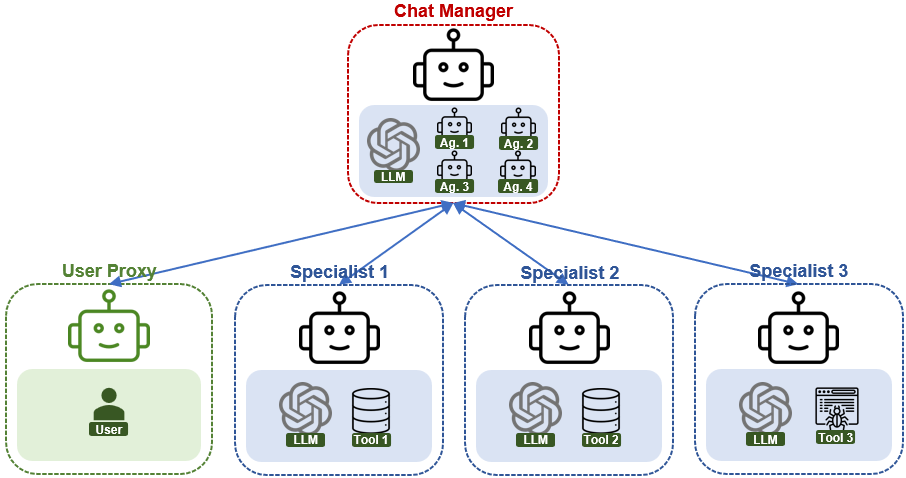
\includegraphics[width=.75\textwidth]{images/agent_config_2.png}
                \caption{Chat setup with one Chat Manager and a group of LLM agents.}
                \label{fig:agent_config_2}
            \end{figure}
            
            
            \begin{figure}[h]
                \centering
                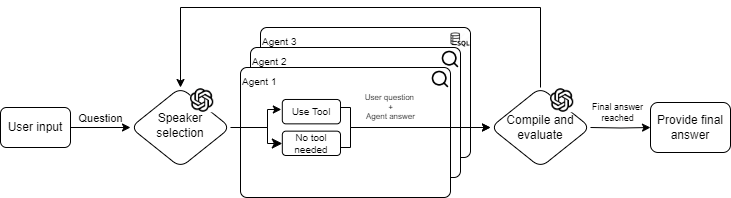
\includegraphics[width=1\textwidth]{images/agent_diagram_2.png}
                \caption{Multi-agent decision process.}
                \label{fig:diagrama_agente_MultiAgente_2}
            \end{figure}

            
        \subsection{Evaluation.}             

            For the evaluation process, in line with the evaluation conducted by \citep{Li2023}, a group of 3 specialist engineers analyzed 33 questions\xexeo{Coloca todas na tabela! E faz uma seção de criação de perguntas, ou subseção} and their corresponding answers for each configuration. 
            The experts assessed each Q\&A pair based on the following predefined metrics:

            \begin{itemize}
                
                \item \textbf{Truthfulness:} a metric to gauge the extent of divergence from factual accuracy.\xexeo{tem que descrever em mais detalhes e de onde tirou}
        
                \item  \textbf{Performance:} encompasses the overall quality of responses, considering linguistic coherence, logical reasoning, diversity, and the presence of corroborative evidence.\xexeo{tem que descrever em mais detalhes e de onde tirou}
                
            \end{itemize}
            
            The final grade was determined by averaging the scores of the all entries for each configuration. This evaluation ensured a comprehensive assessment of the models' capabilities.





\section{Proposed Artefacts}
\todo[inline]{Nessa seção descreve as soluções que você criou (pega do texto que já tem}
\subsection{Single-Agent Solution}
\subsection{Multi-Agent Solution}

            
    \section{Results}

    \todo[inline]{Em vez de Results, evaluation?, e você descreve como os artefatos foram avaliados, o texto que tem está bom, é só reorganizar}

\subsection{Data Set Creation}

\todo[inline]{Aqui descreve todo o seu processo de criação das perguntas e todas elas, que tipo são, faz o máximo que puder. Isso é bem legal.}

\subsection{Metrics}

\todo[inline]{Tem que descrever na revisão da literatura de forma geral, mas se forem diferentes por experimento, tem que explicitar aqui as que vai usar.}


        This section provides an analysis of the data collected and answers the research questions. The results are presented in \autoref{tab:tabela_resultados} and are organized according to the objectives of the study, with each objective being addressed in detail.

        The third metric, LLM Cost\xexeo{Isso aqui é uma pergunta de pesquisa tem que entrar de alguma maneira na definição do DSR, lembrando que as avaliações do DSR podem ser mais de uma}, represents\xexeo{Não é represents, já que é o custo mesmo, acho que  corresponds to, ou mesmo só is } the financial cost associated with using OpenAI's API for the language models in each configuration. This metric is measured in US dollars and reflects the computational resources required for each task.\xexeo{Tem que falar alguma coisa que não é o único custo, e quais são os outros e porque esse é importante, isso pode estar descrito no modelo DSR, antes}\xexeo{Esse parágrafo tipicamente aparece na revisão}
                
            
        \begin{table}[h]
            \small % Reduce the font size
            \centering % Center the table on the page
            \caption{Results on Q\&A and Text-to-SQL tasks, including standard deviation (Std). The best metrics are highlighted with \textbf{\underline{bold and underline}}. The second best are highlighted with \textbf{bold}.}
            \label{tab:tabela_resultados}
            \begin{tabular}{|>{\raggedright\arraybackslash}p{2.2cm}|>{\centering\arraybackslash}p{0.9cm}|>{\centering\arraybackslash}p{0.8cm}|>{\centering\arraybackslash}p{0.8cm}|>{\centering\arraybackslash}p{0.8cm}|>{\centering\arraybackslash}p{0.8cm}|>{\centering\arraybackslash}p{0.8cm}|>{\centering\arraybackslash}p{0.9cm}|>{\centering\arraybackslash}p{0.8cm}|>{\centering\arraybackslash}p{0.8cm}|>{\centering\arraybackslash}p{0.8cm}|}
                \hline
                \rowcolor{gray!20}
                \textbf{Task}           & \multicolumn{5}{c|}{\textbf{Single-Agent}}           & \multicolumn{5}{c|}{\textbf{Multi-Agent}} \\ % Merging cells and adding heading
                \textbf{Model}          & \textbf{LLM Cost} & \textbf{Truth.} & \textbf{Std} & \textbf{Perf.} & \textbf{Std} & \textbf{LLM Cost} & \textbf{Truth.} & \textbf{Std} & \textbf{Perf.} & \textbf{Std} \\ \hline
                \cellcolor{gray!20} Q\&A & & & & & & & & & &\\
                GPT-3.5-turbo            & 0.005             & 2.94              & 1.48 & 3.94          & 1.09 & 0.02              & 4.09              & 1.22 & 3.82 & 0.98 \\
                GPT-4                   & 0.12              & \textbf{3.88}     & 1.41 & \textbf{4.06} & 1.30 & 0.45              & \underline{\textbf{4.57}} & 0.79 & \underline{\textbf{4.43}} & 0.79 \\
                \cellcolor{gray!20} Text-to-SQL & & & & & & & & & &\\
                GPT-3.5-turbo            & 0.009             & 4.13              & 1.41 & 4.44          & 1.03 & 0.02              & \textbf{4.29}     & 1.20 & \textbf{4.29} & 1.33 \\
                GPT-4                   & 0.10 & \underline{\textbf{4.56}} & 0.96 & \underline{\textbf{4.63}} & 0.81 & 0.51      & 3.20              & 1.99 & 3.70 & 1.89 \\ \hline
            \end{tabular}
        \end{table}

        % A análise comparativa entre as arquiteturas de agentes únicos e multiagentes para o RAG, utilizando modelos GPT-3.5-turbo e GPT-4, revelou insights em relação as métricas de truthfulness, performance e custos do modelo de linguagem. 
        The comparative analysis between single and multi-agent setups for RAG, using GPT-3.5-turbo and GPT-4 models, revealed insights regarding the metrics of truthfulness, performance, and costs of the language model.

        
        \subsection{Truthfulness} 
            % Na avaliação da métrica truthfulness, observa-se diferenças significativas entre as configurações de agente único e multi-agente em ambas as tarefas de Q\&A e Text-to-SQL. Os resultados são ilustrados nas Figuras ~\ref{fig:truthfulness_QA} e ~\ref{fig:truthfulness_text2sql}.
            In assessing the truthfulness metric, significant differences are noted between the single and multi-agent settings in both Q\&A and Text-to-SQL tasks. The results are illustrated in Figures \ref{fig:truthfulness_QA} and \ref{fig:truthfulness_text2sql}.
            For Q\&A tasks, GPT-4 in a multi-agent configuration significantly exceeded the performance of the single-agent with a truthfulness score of 4.57 compared to 3.88. The GPT-3.5-turbo model showed distinct results between the two configurations, with the multi-agent surpassing the single-agent with scores of 4.09 and 2.94, respectively.
            In terms of Text-to-SQL queries, a different outcome was observed. GPT-4 single-agent achieved a score of 4.56, while the same model in the multi-agent configuration obtained 3.20, highlighting a limitation for the multi-agent in this task. Conversely, the GPT-3.5-turbo maintained a more balanced performance between configurations, scoring 4.29 for multi-agent and 4.13 for single-agent.
            
            
            
            \begin{figure}[h]
                \centering
                \begin{minipage}{.49\textwidth}
                    \centering                
                    % \framebox{
                    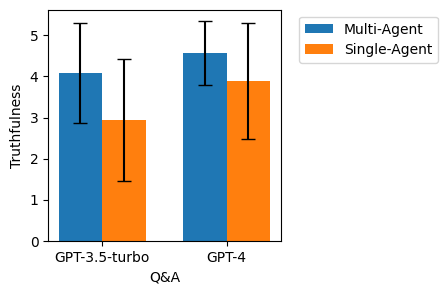
\includegraphics[width=1\linewidth]{images/truthfulness_QA.png}
                    % }
                    \caption{Truthfulness and standard deviation in Q\&A tasks by LLM model and agent configuration. \\ }
                    % \caption{Truthfulness and standard deviation in Q\&A tasks by LLM model and agent configuration.}
                    \label{fig:truthfulness_QA}
                \end{minipage}%
                \hspace{0.2cm}
                \begin{minipage}{.49\textwidth}
                    \centering
                    % \framebox{
                    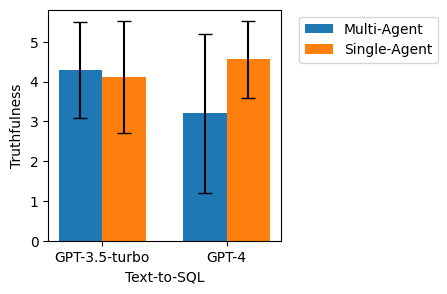
\includegraphics[width=1\linewidth]{images/truthfulness_text2sql.png}
                    % }
                    \caption{Truthfulness and standard deviation in Text-to-SQL tasks by LLM model and agent configuration.}
                    \label{fig:truthfulness_text2sql}
                \end{minipage}
            \end{figure}

            
            
            
        \subsection{Performance}        
        
            The evaluation of LLM performance \citep{Li2023} in the tasks of Q\&A and Text-to-SQL reveals trends which are similar to the truthfulness results. 
            As shown in Figures \ref{fig:performance_QA} and \ref{fig:performance_text2sql} and summarized in \ref{tab:tabela_resultados}, the text performance in single and multi-agent setups was compared using the GPT-3.5-turbo and GPT-4 models.        
            For Q\&A tasks, the multi-agent setup shows a performance boost compared to the single-agent setup. In particular, the multi-agent GPT-4 achieves a performance score of 4.43, which is higher than the single-agent GPT-4 score of 4.06. This pattern is consistent with the GPT-3.5-turbo, where the multi-agent system also surpasses the single-agent system, scoring 3.82 and 3.94, respectively. These findings emphasize the effectiveness of the multi-agent approach in handling technical user queries.
                    
            \begin{figure}[h]
                \centering
                \begin{minipage}{.48\textwidth}
                    \centering                
                    % \framebox{
                        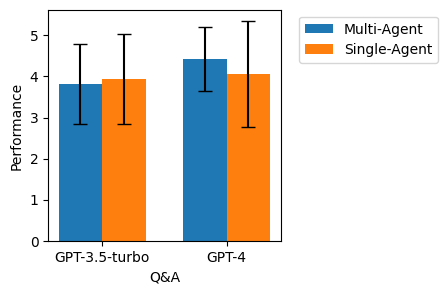
\includegraphics[width=1\linewidth]{images/performance_QA.png}
                    % }
                    \caption{Performance and standard deviation in Q\&A tasks by LLM model and agent configuration.\\}
                    % \caption{Performance and standard deviation in Q\&A tasks by LLM model and agent configuration.}
                    \label{fig:performance_QA}
                \end{minipage}
                \hspace{0.2cm}
                \begin{minipage}{.48\textwidth}
                    \centering
                    % \framebox{
                    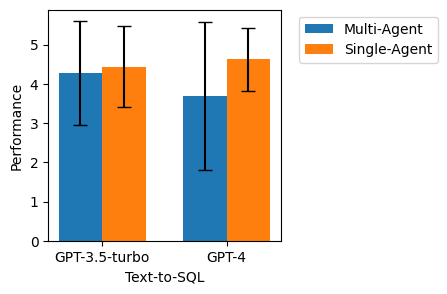
\includegraphics[width=1\linewidth]{images/performance_text2sql.png}
                    % }
                    \caption{Performance and standard deviation in Text-to-SQL tasks by LLM model and agent configuration.}
                    \label{fig:performance_text2sql}
                \end{minipage}%
            \end{figure}

        % \subsection{Tempo de Resposta}
        
            % O tempo médio de resposta dos agentes foi registrado, mostrando uma resposta rápida para a maioria das perguntas. No entanto, algumas consultas mais complexas exigiram tempos de processamento mais longos.
            
        % \subsection{LLM Cost}
        
        \subsection{LLM Cost} 
            Language model services are typically composed by a values per token. For instance, GPT-4 model costs US\$30.00 (input) and US\$60.00 (output) per 1 million tokens received and sent, respectively.        
            The single-agent architecture demonstrated substantially lower costs for both Q\&A and Text-to-SQL tasks compared to the multi-agent setup as shown in Figure~\ref{fig:truthfulness_vs_cost_vs_config_model}. For instance, the average cost of the GPT-4 model \citep{OpenAI2023} for a Q\&A task was \$0.12 per processed question for the single-agent, while the multi-agent recorded an average cost of \$0.45. This trend of higher costs for the multi-agent architecture was also maintained for Text-to-SQL tasks, with an average cost of \$0.51 for the multi-agent architecture in contrast to \$0.10 for the single agent.
            The higher token count and cost for multi-agent setting is due to the inclusion of intermediate calls, for example, when the "Agent Selector" needs to decide which agent to pass the turn to. All the message history is passed to the LLM at this stage, substantially increasing the number of tokens submitted and response time.
        

            \begin{figure}[h]
                \centering              
                % \framebox{
                    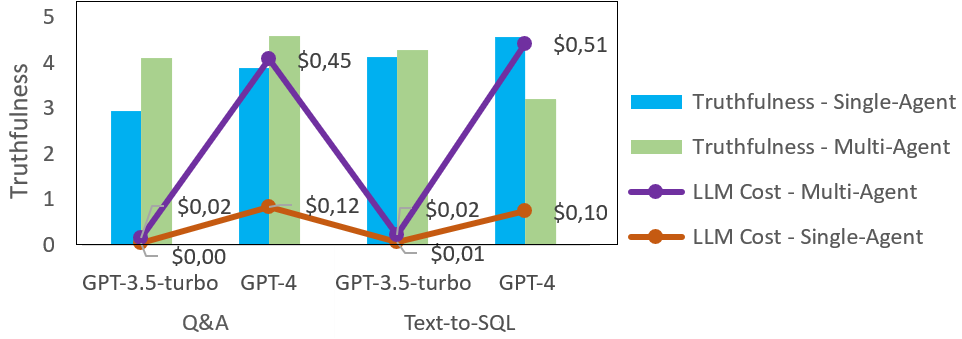
\includegraphics[width=0.75\textwidth]{images/truthfulness_vs_cost_vs_config_model.png}
                % }
                \caption{Average LLM costs and Truthfulness per completed task according to setup and model.}
                \label{fig:truthfulness_vs_cost_vs_config_model}
            \end{figure}
            
            

    \section{Discussion}

        The comparison between single and multi-agent systems revealed significant differences in terms of performance and cost:
        
        \subsection{General Performance.}     
            The results indicate that for Q\&A tasks in the context of O\&G, truthfulness measure was 28\% higher with the multi-agent architecture compared to single. 
            However, for Text-to-SQL tasks, this trend was inverted, where the single-agent scored 15\% higher.

            These findings suggest that for Q\&A tasks, the multi-agent setup may be more advantageous in terms of providing truthful information, particularly when utilizing the more advanced GPT-4 model. 
            Conversely, in Text-to-SQL tasks, the GPT-4 model in a single-agent configuration proved more effective. 
            This might imply that the added complexity of managing multiple agents in some tasks does not necessarily lead to improved performance in responses, underscoring the importance of carefully selecting the agent configuration based on the task type and specific features of the language model used.
                
        \subsection{Cost-Performance Analysis.}
            While the multi-agent system shows higher truthfulness in Q\&A tasks, it is crucial to consider the associated costs. 
            % For instance, a truthfulness score of 3.8 in a multi-agent setup might be acceptable if the cost is significantly lower than achieving a 4.5 score with a single-agent system. 
            % Based on our analysis, we recommend using a multi-agent system for Q\&A tasks when the budget allows for it and truthfulness is a critical factor. For Text-to-SQL tasks, a single-agent system is preferable due to its higher performance and potentially lower cost. Decision-makers should consider setting a cost-performance threshold to guide the choice of system configuration, ensuring that the benefits justify the expenses involved.
            To provide a clearer comparison, let us consider the score/cost ratios. For Q\&A tasks using GPT-4, the single-agent configuration yields a ratio of 32.33 truthfulness points per dollar, compared to 10.16 for the multi-agent setup. This indicates that while the multi-agent system shows a 17.8\% improvement in truthfulness, it comes at a 275\% increase in cost.
            
            Based on our analysis, we recommend using a multi-agent system for Q\&A tasks when the budget allows for it and accuracy is a critical factor. 
            However, decision-makers should consider setting a cost-performance threshold to guide the choice of system configuration, ensuring that the benefits justify the expenses involved.\xexeo{TEm que deduzir a necessidade de fazer um experimento antes levando essas coisas em consideração}


        \subsection{Model Performance Variations.}
            Interestingly, our results show that GPT-3.5-turbo outperforms GPT-4 in certain tasks, particularly in the Text-to-SQL multi-agent configuration, despite GPT-4's larger size and more extensive training. 
            This unexpected performance could be attributed to several factors. 
            First, GPT-3.5-turbo may have undergone more specific fine-tuning for structured query tasks, allowing it to excel in Text-to-SQL scenarios. 
            Additionally, GPT-3.5-turbo's training data might be more recent or more relevant to the specific domain of our study. 
            Another possibility is that the smaller model size of GPT-3.5-turbo allows for faster processing and more efficient handling of the multi-agent setup, resulting in better performance in some contexts.

            However, it is important to note that GPT-4, when used in a multi-agent setup, demonstrated more consistent truthfulness and performance, as evidenced by its reduced standard deviation in results. 
            This consistency can be particularly advantageous in applications where reliability and accuracy are critical. 
            Multi-agent systems have the advantage of maintaining separate contexts for different aspects of a task. \xexeo{Você pode suportar essa afirmação com uma citação?}
            This compartmentalization can lead to better handling of complex, multi-faceted queries, as each agent can focus on its specific context without being overwhelmed by irrelevant information. However, this advantage may be offset in tasks like Text-to-SQL, where maintaining a unified context of the database schema and query structure is crucial, possibly explaining the better performance of single-agent setups in this task.
            Furthermore, the multi-agent architecture inherently involves multiple stages of information processing, which can serve as natural filtering mechanisms.
            As information passes from one agent to another, irrelevant or low-quality data may be naturally filtered out, leading to more refined and accurate final outputs. 
            This could explain the superior performance in filtering irrelevant information observed in multi-agent setups.
        
        
        \subsection{Economic Efficiency.} 
            % The multi-agent architecture demonstrated a cost, on average, 3.7 times higher than that of the single-agent. This increase is due to the addition of intermediate calls to the language model, for instance, in the Speaker Selection phase, where a request is necessary to select the next agent for dialogue. Additionally, more than one iteration between agents for action planning and tool use can occur. From the model standpoint, the average cost of completed tasks (from user question to final answer) using GPT-4 was 21 times higher than those performed with GPT-3.5-turbo, an expected difference due to the varying costs of each service.
            The multi-agent architecture incurs significantly higher costs compared to the single-agent system, primarily due to additional intermediate calls to the language model and multiple iterations between agents for action planning. 
            Also, the cost differences between using GPT-4 and GPT-3.5-turbo are substantial, with GPT-4 being notably more expensive\xexeo{Dizer x vezes mais caro em julho de 2025}.
            As detailed in the Cost-Performance Analysis section, the truthfulness per dollar ratio highlights the economic trade-offs between single-agent and multi-agent systems. While the multi-agent system offers improvements in truthfulness, this comes at a considerable increase in cost, impacting the overall economic efficiency.
            
            % To provide a clearer picture of economic efficiency for a large company with 40.000 knowledge workers, using GPT-4 could result in an annual cost of approximately \$5M, while GPT-3.5-turbo would cost around \$500.000. These estimates assume an average usage pattern of 10.000 tokens per worker per day and highlight the significant impact of model choice on operational costs.
            % To provide a clearer picture of economic efficiency, we can examine the truthfulness per dollar ratio. The single-agent system yields 32.33 truthfulness points per dollar, whereas the multi-agent system yields 10.16 truthfulness points per dollar. This comparison highlights that, although the multi-agent system shows a 17.8\% improvement in truthfulness, it comes at a 275\% increase in cost, resulting in a lower truthfulness per dollar ratio compared to the single-agent system.

            % For a large company with 40,000 knowledge workers, using GPT-4 could result in an annual cost of approximately \$5M, while GPT-3.5-turbo would cost around \$500,000. These estimates assume an average usage pattern of 10,000 tokens per worker per day and highlight the significant impact of model choice on operational costs.
            For a large company with 40,000 knowledge workers, the choice of model and architecture significantly impacts annual costs. 
            Using GPT-4 in a single-agent configuration could result in an annual cost of approximately \$4.38 million, while GPT-3.5 would cost around \$438,000. However, when employing a multi-agent architecture, the costs increase substantially. \xexeo{Pulou como você chegou a esses números, eu estou achando até baixos, qual a conta que você fez (empregados x consultas x etc...)}
            The multi-agent configuration with GPT-4 would escalate the annual cost to \$16.425 million, representing a dramatic increase due to the 3.75 times higher token usage. 
            Similarly, GPT-3.5 in a multi-agent setup would cost \$1.642 million. 
            These estimates assume an average usage pattern of 10,000 tokens per worker per day and underscore the significant financial implications of adopting a multi-agent system, which, while potentially offering performance benefits, comes with a considerable increase in LLM costs.\xexeo{Ah! Tá no fim do parágrafo e precisa ser no início. Além disso tem que dizer quantos dias de trabalho por ano, e o custo de cada token em uma data}

            In summary, while multi-agent systems and more advanced models like GPT-4 offer improvements in performance, the economic efficiency, as measured by truthfulness per dollar, may favor single-agent systems and less costly models like GPT-3.5-turbo, depending on the specific application and budget constraints.\xexeo{In summary é o parágrafo típico das LLMs... Mas é isso mesmo. Porém tem que colocar um ponto: o custo dos modelos está caindo barbaramente com o aparecimento de novos modelos no topo de desempenho e novas tecnologias tem permitido alcançar resultados de ótima qualidade com máquinas muito menores, o que também derruba o custo. Pode até citar o exemplo do DeepSeek (buscando na literatura o desempenho x custo dele}
            
        % \subsection{Challenges and Limitations}
        
        \subsection{Challenges and Limitations.}     
            During the evaluation of the agents, several challenges and limitations were identified.

            \setlength{\parindent}{1em}
            \textbf{\textit{Contextualization and Interpretation.}} 
                In many cases, the single-agent solution had difficulty understanding the context of the question. For example, a question about cementing was interpreted in the context of the construction industry, a theme to which the language models were more exposed during the training phase. 
                However, the multi-agent structure, with its well-defined roles, better understood the questions and showed superior performance in Q\&A tasks, corroborating the findings of \citep{Li2024}.
            
            \setlength{\parindent}{1em}
            \textbf{\textit{Filtering Irrelevant Information.}} 
                The agent often receives irrelevant documents along with important ones in the prompt context, and it is up to the LLM to ignore these. 
                For example, when asked about alternatives to accelerate the curing time of cement paste without compromising its integrity at high temperatures, the RAG system retrieved a document that included information about batch cementing to ensure homogeneity during manufacturing and pumping. 
                While this information is true, it was not relevant to the specific question asked. 
                In this aspect, the multi-agent solution performed better at discarding such irrelevant information, focusing more accurately on the task at hand. 
                Other possible solutions include improving the accuracy of semantic search by adjusting a minimum threshold for similarity measures or through re-ranking techniques such as those proposed by \citep{Carraro2024} and \citep{Sun2023}.
            
            \setlength{\parindent}{1em}
            \textbf{\textit{Hallucination.}} 
                During the evaluation of our system, we encountered instances where the agent produced hallucinated information instead of utilizing the appropriate tool to retrieve accurate data, as in \citep{Bilbao2023}. 
                For example, when asked, "How many anomalies occurred on rig number 05 during August 2023?" the agent was expected to use the Text-to-SQL tool to query the database. 
                However, it bypassed this tool and generated a fabricated response, stating that 5 anomalies occurred, along with detailed descriptions of fictional events. The correct answer, as retrieved from the database, was that 7 anomalies occurred. This hallucination likely resulted from the agent's reliance on its internal knowledge rather than external data retrieval. 

                In terms of hallucination statistics, our analysis revealed that for Q\&A tasks, hallucinations occurred in 9.6\% of cases and 3.8\% for partially hallucinated. 
                In contrast, Text-to-SQL tasks exhibited a lower hallucination rate, with only 3.6\% of responses containing hallucinated information and 96.4\% being accurate. 
                These findings highlight the variation of susceptibility to hallucination in different types of tasks, highlighting the need for targeted strategies to mitigate this problem.
            
            \setlength{\parindent}{1em}
            \textbf{\textit{Industry Jargon:}}
                Specifically analyzing the activity of drilling and completion of offshore wells, the main challenge is the inherently complex and technical nature of the data involved. 
                There were instances of incorrect interpretation of information, likely due to the use of terms, expressions, and themes specific to well construction, to which the language model had little or no exposure during training phase. 
                A possible solution is the implementation of specialized models, which has been pointed out in gray literature as a trend for the coming years \citep{Shah2024, Meena2023, Ghosh2023}.
            
            \setlength{\parindent}{1em}
            \textbf{\textit{Tools vs. Performance:}} 
                It was identified during the experiments that agents with a high amount of tools showed a decline in overall performance. 
                This can be attributed to the added context to the prompts. 
                As the context length increases, the model's ability to accurately interpret and respond diminishes.
                This is a limitation of current language models, where longer contexts can lead to a dilution of relevant information and increased difficulty in maintaining coherence and accuracy. 
                This conclusion is currently qualitative, as these metrics were not addressed in this experiment.

            
            \setlength{\parindent}{1em}
            \textbf{\textit{Queries Involving Proper Names:}}
                In queries involving people's names, it was not possible to retrieve relevant documents using semantic search. 
                For example, when asked to identify the employee associated with a specific key and list knowledge items they registered in the system, the RAG system incorrectly attributed knowledge items to the wrong author\xexeo{O RAG ou a LLM usando o RAG, não ficou claro}. 
                This highlights the difficulty in accurately retrieving information based on proper names, which can be complicated by variations in accentuation, abbreviation, and formatting.\xexeo{tem evidências disso em outros artigos?}
                A potential solution to be explored is the use of Self-Query Retriever \citep{LangchainSelfQuery2023}, implementing a hybrid search with metadata filters (including proper names) and semantic retrieval of the rest of the query. 
                It is also suggested, in these cases, to use the \citep{Levenshtein1966} distance to handle possible variations in the spelling of names. 
                This approach could improve the accuracy of retrieving documents related to specific individuals, ensuring that the correct information is associated with the right person.
                
        
        % \subsection{Practical Implications}
        \subsection{Practical Implications.} 
                    The findings from our study have significant practical implications for the O\&G sector, and potentially for other industries characterized by complex and technical data environments:
                    
                \begin{itemize}
                
                    \item \textbf{Enhanced Decision-Making Support:}
                        Our results indicate that multi-agent systems provide a 28\% higher truthfulness measure in Q\&A tasks. This can be particularly beneficial for decision-making in well engineering, where accurate and truthful information is critical.
                        Implementing multi-agent systems in decision-making processes can lead to more reliable and informed decisions, thereby reducing the risk of errors and enhancing operational safety and efficiency.
                    
                    \item \textbf{Balancing Performance and Economic Efficiency:}
                        While multi-agent systems offer superior performance in terms of truthfulness, they come with a cost that is 3.7 times higher on average compared to single-agent systems.
                        This highlights the importance of a strategic approach in selecting agent configurations based on specific tasks and budget constraints. 
                        % For instance, single-agent systems might be more cost-effective for Text-to-SQL tasks where they have shown to perform 15\% better. 
                        A detailed cost-benefit analysis reveals that for Q\&A tasks using GPT-4, the single-agent configuration yields a ratio of 32.33 truthfulness points per dollar, compared to 10.16 for the multi-agent setup. While the multi-agent system shows a 17.8\% improvement in truthfulness, this comes at a 275\% increase in cost. The efficiency varies significantly by task type; in Text-to-SQL tasks, the GPT-4 single-agent outperforms the multi-agent by 42.5\% in truthfulness while costing 80.4\% less. 
                        % These quantitative insights emphasize the need for careful consideration of task requirements and budget constraints when choosing between single and multi-agent configurations.
                        
                    \item \textbf{Reflection and Critic Agents:}
                        A promising approach to enhance the performance of these agents is the use of reflection \citep{Shinn2023}, a method where agents verbally reflect on task feedback signals and maintain this reflective text in an episodic memory buffer to improve decision-making in subsequent trials. Critic agents are a way to implement reflection in a multi-agent setup. This type of agent is challenging to apply in Q\&A tasks over private technical data, as commercial LLMs (OpenAI, Google Bard, and others) have not been deeply trained in the domain and struggle to provide relevant and precise critiques, reinforcing the trend toward increased use of domain-specific models \citep{Shah2024, Meena2023, Ghosh2023}.                
                        
                    \item \textbf{Task-Specific Agent Configuration:}
                        The study highlights that the complexity of managing multiple agents does not always lead to better performance. In some cases, a single-agent setup might be more effective.
                        This insight can guide the development and deployment of AI systems, ensuring that the configuration of agents is tailored to the specific requirements of the task, thereby optimizing both performance and cost.           
                        
                    \item \textbf{Potential for Broader Application:}
                        The insights gained from this study are not limited to the O\&G sector but can be applied to other industries with similar technical complexities, such as aerospace, pharmaceuticals, and renewable energy.
                        By adopting multi-agent systems in these industries, organizations can improve decision-making, knowledge management, and operational efficiency, driving innovation and competitiveness.             
                    
                \end{itemize}
                    
                
        \subsection{Future Directions.} 

            This work indicates possible pathways for enhancing RAG architectures in O\&G sector. 
            
            \begin{itemize}
            
                \item \textbf{Enhancement of IR Semantic Techniques:}
                    There is a critical need to develop more sophisticated semantic search technologies. Future efforts should focus on enhancing the precision of information retrieval by filtering out irrelevant content more effectively. This will ensure that agents can provide more accurate and contextually appropriate responses, crucial for technical domains such as O\&G.
                    
                \item \textbf{Development of Domain-Specific Models:}
                    Specialized models tailored specifically to the O\&G and other domains, such as biomedical engineering \citep{Pal2024}, could significantly improve the handling of specific jargon and complex technical data, while reducing LLM costs \citep{Arefeen2024}. Future research should aim to develop and train these models to better understand and interpret the unique language and data types found in O\&G, enhancing the overall accuracy of agent responses.
                    
                \item \textbf{Optimization of Tool Use in Agent Performance:}
                    The relationship between the quantity of tools available to an agent and its performance needs further exploration. Future studies should quantify the impact of tool availability on agent efficacy and efficiency, aiming to optimize tool use without overwhelming the agent or diluting performance quality.
                    
                \item \textbf{Integration of Advanced Name Recognition Techniques:}
                    Queries involving proper names pose a significant challenge in semantic search. Integrating advanced retrieval techniques, such as Self-Query Retrievers \citep{LangchainSelfQuery2023} and \citep{Levenshtein1966} distance algorithms, could improve the handling of these queries. Future research should focus on enhancing name recognition capabilities to ensure that agents can accurately retrieve and utilize correct information, especially in scenarios where precision is paramount.
                    
                \item \textbf{Extension to Other Complex Domains:}
                    The potential applications of multi-agent systems are not limited to the O\&G sector. Future research should explore the adaptation and implementation of these systems in other complex and technical domains, such as aerospace, pharmaceuticals, and renewable energy. Investigating how these systems can support decision-making in these areas will provide valuable insights into their versatility and adaptability.
                    
                \item \textbf{Hybrid Model Experimentation:}
                    Combining the strengths of single and multi-agent systems could yield significant benefits. Future directions should include experimenting with hybrid models that integrate the robustness and depth of multi-agent interactions with the simplicity and efficiency of single-agent systems. This hybrid approach could potentially offer a balanced solution, maximizing performance while managing costs and complexity.
                    

            \end{itemize}
            
            By pursuing these directions, future research can significantly advance the development of multi-agent systems, not only enhancing their application in the O\&G sector but also expanding their utility across various technologically intensive activities.
            